\section{Helper Tools}
In section we explain some tools which are implemented to help developers. This tools help developers to add the support of run-time state migration approach in existing applications.
\subsection{ASML Schema Library}
A repository which hosted on GitHub\footnote{\url{https://github.com/asml-lang/asml}} that contains latest version of Application State Modeling Language abstract syntax which is JSON a Schema document. Also, this repository contains some examples and the DSL manual. Moreover, for ease of implementation this repository published on Node Repository Manager (NPM)\footnote{\url{https://www.npmjs.com/package/asml}}
 and other JavaScript packages are using it as the main schema.
 

\subsection{ASML Editor}
ASML Editor is a playground web application\footnote{\url{https://asml-lang.github.io/asml/editor/}} developed in HTML,CSS, and JavaScript. ASML Editor's purpose is to assist developers write Application State Models and test a Run-Time State. In case of an validation or syntax error in any section, an error box shows up below that section and displays the error description like in Figure \ref{fig:asml-editor}. 
\FloatBarrier \begin{figure}[H]
    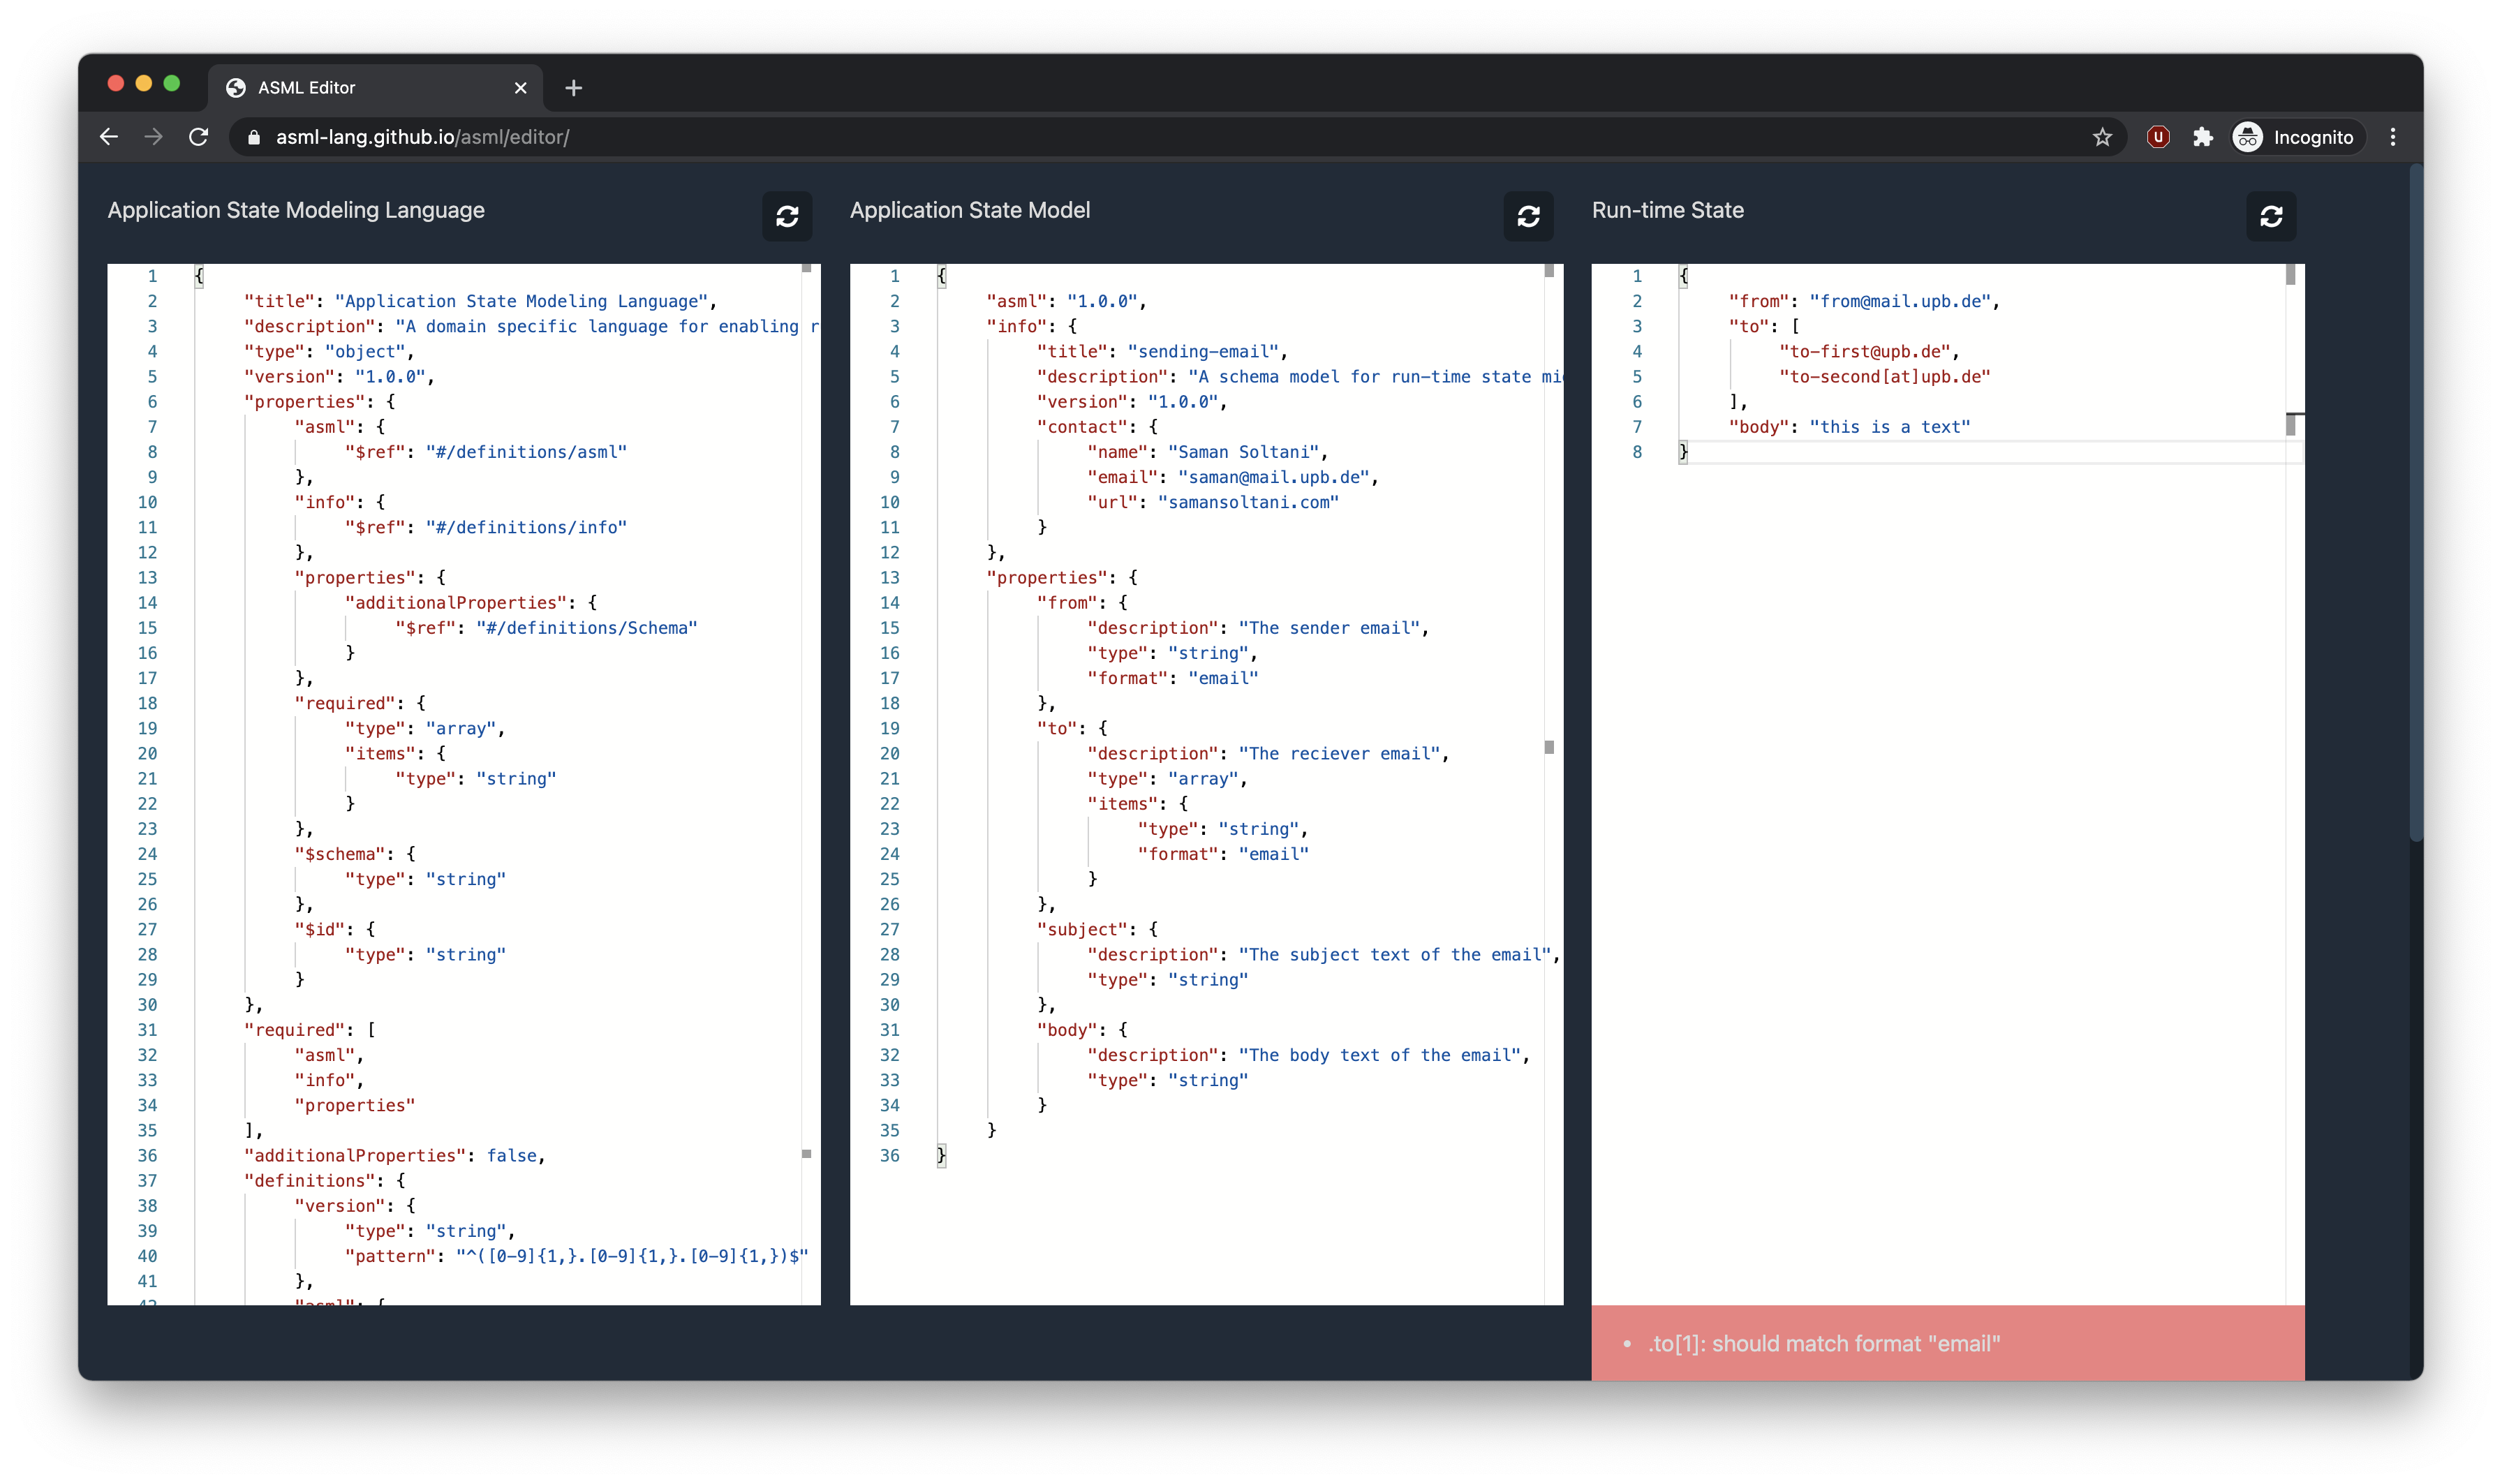
\includegraphics[width=\linewidth]{../figures/asml-editor.png}
    \centering
    \caption{ASML Editor live playground}
    \label{fig:asml-editor}
\end{figure} \FloatBarrier

\subsection{ASML CLI}
ASML CLI is a command-line interface which helps developers to validate Application State Model and generate interfaces based on them for different programming languages. This tool is published on NPM \footnote{\url{https://www.npmjs.com/package/asml-cli}}.

ASML CLI supports interface generating in these programming languages:
Ruby, JavaScript, Flow, Rust, Kotlin, Dart, Python, C\#, Go, C++, Java, TypeScript, Swift, Objective-C, Elm.

\subsection{ASML Validator Library}
ASML Validator is a JavaScript library that allow a JavaScript application validate the Application State Model and Run-time State against Application State Modeling Language. This library using ASML Schema Library as the main schema for validating. The source code of this library is available on GitHub\footnote{\url{https://github.com/asml-lang/asml-validator}}. Also this library is published on NPM\footnote{\url{https://www.npmjs.com/package/asml-validator}} and it is used in Run-time State Migration JavaScript Library, ASML Editor and ASML Command-line Interface.

